\documentclass[UTF8,AutoFakeBold]{ctexart}
\usepackage{fontspec}
\setmainfont{Times New Roman}
% ===========================页面设置===============================================
\usepackage{geometry}   %设置页边距的宏包
\geometry{left=3.2cm,right=3.2cm,top=4cm,bottom=3cm}  %设置 上、左、下、右页边距
% ===========================基础设置===============================================
\usepackage{graphicx}  %插入图片的宏包
\usepackage[colorinlistoftodos]{todonotes} %插入to-do
\usepackage{float} %设置图片浮动位置的宏包 
\usepackage{subfigure} %插入多图时用子图显示的宏包
\usepackage{xcolor}
\usepackage[colorlinks=true]{hyperref} %超链接,支持unicode字符
\hypersetup{
    colorlinks,
    linkcolor={red!50!black},
    citecolor={blue!50!black},
    urlcolor={blue!80!black}
}
\usepackage{indentfirst} %设置缩进
\setlength{\parindent}{2em} %也可在正文中非全局设置
\usepackage{mdframed} %frame
\mdfdefinestyle{mdfexample}{
    innertopmargin=-1pt,
    innerleftmargin=1cm,
    innerrightmargin=2cm,
    roundcorner=30pt,
    linecolor=green!20,
    linewidth=2pt,
    backgroundcolor=gray!20,
    frametitlerule=true,
    frametitlebackgroundcolor=grey!40!white
}
\usepackage{listings} %插入代码块
\definecolor{codegreen}{rgb}{0,0.6,0}
\definecolor{codegray}{rgb}{0.5,0.5,0.5}
\definecolor{codepurple}{rgb}{0.58,0,0.82}
\definecolor{backcolour}{rgb}{0.95,0.95,0.92}

\lstdefinestyle{mystyle}{
    backgroundcolor=\color{backcolour},       % 设定背景颜色
    commentstyle=\color{codegreen},           % 设定注释颜色
    keywordstyle=\color{magenta},             % 设定关键词颜色
    numberstyle=\tiny\color{codegray},        % 设定行号格式
    stringstyle=\color{codepurple},           % 设定字符串格式
    basicstyle=\ttfamily\footnotesize,        % 设定代码字号
    breakatwhitespace=false,                  % sets if automatic breaks should only happen at whitespace
    breaklines=true,                          % sets automatic line breaking
    captionpos=b,                             % 设定说明位置
    keepspaces=true,                 
    numbers=left,                             % 设定行号在左边
    numbersep=5pt,                            % 设定行号与代码间距
    showspaces=false,                         
    showstringspaces=false,
    showtabs=false,                  
    tabsize=4
}
\def\cmd#1{\texttt{\color{red}\footnotesize $\backslash$#1}}
\def\env#1{\texttt{\color{blue}\footnotesize #1}}
\definecolor{deepblue}{rgb}{0,0,0.5}
\definecolor{deepred}{rgb}{0.6,0,0}
\definecolor{deepgreen}{rgb}{0,0.5,0}
\definecolor{halfgray}{gray}{0.55}

\lstdefinestyle{anotherstyle}{
    basicstyle=\ttfamily\footnotesize,
    keywordstyle=\bfseries\color{deepblue},
    emphstyle=\ttfamily\color{deepred},    % Custom highlighting style
    stringstyle=\color{deepgreen},
    numbers=left,
    numberstyle=\small\color{halfgray},
    rulesepcolor=\color{red!20!green!20!blue!20},
    frame=shadowbox,
}
%%%设置页眉与页脚%%%
\usepackage{fancyhdr}
\pagestyle{fancy}
\fancyhf{}
\setlength{\headheight}{12.64723pt}
\addtolength{\topmargin}{-0.64723pt}
\lhead{\fangsong 实习总结}
\rhead{\fangsong 张悟生}
\cfoot{\thepage}

\renewcommand{\headrulewidth}{1pt}

%%%% 下面的命令设置行间距与段落间距 %%%%
\setlength{\parskip}{1.0em} %设置段间距
\setlength{\baselineskip}{1.3em} %设置行间距

%文章内中文自动换行,可以自行调节
\XeTeXlinebreaklocale “zh” %按照中文断行
\XeTeXlinebreakskip = 0pt plus 0.5pt minus 0.1pt %设置字符间距



% ===========================数学符号=============================================== 
\usepackage{amsmath,amsthm,amssymb,bbm} 
\usepackage{cleveref} %引用定理与公式

% ===========================字号===============================================
\newcommand{\chuhao}{\fontsize{42pt}{\baselineskip}\selectfont}
\newcommand{\xiaochuhao}{\fontsize{36pt}{\baselineskip}\selectfont}
\newcommand{\yihao}{\fontsize{28pt}{\baselineskip}\selectfont}
\newcommand{\erhao}{\fontsize{21pt}{\baselineskip}\selectfont}
\newcommand{\xiaoerhao}{\fontsize{18pt}{\baselineskip}\selectfont}
\newcommand{\sanhao}{\fontsize{15.75pt}{\baselineskip}\selectfont}
\newcommand{\sihao}{\fontsize{14pt}{\baselineskip}\selectfont}
\newcommand{\xiaosihao}{\fontsize{12pt}{\baselineskip}\selectfont}
\newcommand{\wuhao}{\fontsize{10.5pt}{\baselineskip}\selectfont}
\newcommand{\xiaowuhao}{\fontsize{9pt}{\baselineskip}\selectfont}
\newcommand{\liuhao}{\fontsize{7.875pt}{\baselineskip}\selectfont}
\newcommand{\qihao}{\fontsize{5.25pt}{\baselineskip}\selectfont}

\renewcommand{\normalsize}{\fontsize{12pt}{\baselineskip}\selectfont}

%%%% 设置 section 属性 %%%%
\ctexset{
    section = {
        %foramt用于设置章节标题全局格式,作用域为标题和编号 
        format={\xiaosihao \bfseries \heiti \raggedright},
        %number用于设置章节编号数字输出格式
        %输出section编号为中文
        number={\chinese{section}、},
        %name用于设置章节号前后的词语
        %前、后词语用英文状态下,分开
        %如果没有前后词语可以不填
        name={},
        %beforeskip用于设置章节标题前的垂直间距
        %ex为当前字号下字母X的高度
        %基础高度为1.0ex,可以伸展到1.2ex,也可以收缩到0.8ex
        beforeskip={-1.0ex plus 0ex minus 0.4ex},
        %afterskip用于设置章节标题后的垂直间距
        afterskip={-0.5ex plus 0.4ex minus 0.2ex},
        %aftername用于控制编号与标题的间距
        aftername={\hspace{0pt}},
    }
}

\ctexset{
    subsection={
        format={\xiaosihao \bfseries \heiti},
        number={\chinese{section}},
        name={(,)},
        beforeskip={-1.0ex plus 0ex minus 0.4ex},
        afterskip={-0.5ex plus 0.4ex minus 0.2ex},
        aftername={\hspace{0.5em}},
    }      
}

\ctexset{
    subsubsection={
        format ={\xiaosihao \bfseries \heiti}, 
        number={\arabic{subsubsection}、},
        beforeskip={-1.0ex plus 0ex minus 0.4ex},
        afterskip={-0.5ex plus 0.4ex minus 0.2ex},
        aftername={\hspace{0pt}},
        }
}

%%%% 定理类环境的定义 %%%%
\newtheorem{example}{例}             % 整体编号
\newtheorem{algorithm}{算法}
\newtheorem{theorem}{定理}[section]  % 按 section 编号
\newtheorem{definition}{定义}
\newtheorem{axiom}{公理}
\newtheorem{property}{性质}
\newtheorem{proposition}{命题}
\newtheorem{lemma}{引理}
\newtheorem{corollary}{推论}
\newtheorem{remark}{注解}
\newtheorem{condition}{条件}
\newtheorem{conclusion}{结论}
\newtheorem{assumption}{假设}

%%%% 重定义 %%%%
%设置目录格式
\usepackage[toc]{multitoc} %双栏排版
\renewcommand{\contentsname}{\bfseries 目录}  % 将Contents改为目录
\renewcommand{\abstractname}{摘要}  % 将Abstract改为摘要
\renewcommand{\refname}{参考文献}   % 将References改为参考文献
\renewcommand{\indexname}{索引}
\renewcommand{\figurename}{图}
\renewcommand{\tablename}{表}
\usepackage[titletoc]{appendix} %插入附录
\renewcommand{\appendixname}{\bfseries 附录}
\renewcommand{\algorithm}{算法}

%%%% 其它配置 %%%%
\usepackage[normalem]{ulem} %插入各种各校的下划线
\usepackage{multirow,multicol,booktabs,longtable,colortbl,array,makecell} %一些关于表格的设置
\usepackage{zhlipsum} %插入一些无聊的文字
\usepackage{comment} %将一段文字变成注释
\usepackage{cancel}
\usepackage{subfiles} % 插入分文档
\usepackage[bottom]{footmisc}



% ===========================正正正正正正正==============================================
% ===========================文文文文文文文===============================================
% ===========================这这这这这这这===============================================
% ===========================里里里里里里里===============================================
% ===========================开开开开开开开===============================================
% ===========================始始始始始始始===============================================
% ===========================写写写写写写写===============================================
% ===========================哟哟哟哟哟哟哟===============================================



\begin{document}
\subfile{titlepage.tex}
\thispagestyle{empty}
\newpage 
\tableofcontents
\thispagestyle{empty}
\newpage 

\pagenumbering{arabic}
\setcounter{page}{1}
\section{写在前面}
这一篇文字,总结我作为一个实习生,在这段时间,\textcolor{red}{也就是从10月8日到12月31日},所做过的工作。
在领导的指导、关心下,在同事们的
帮助、配合下,我学习了许多经验,并帮助同事完成了许多工作,也认识到自己的不足,
为了总结经验,吸取教训,现将我这一段时间的工作总结如下。
\section{关于工作的态度}
态度决定一切,作为一个实习生,如果不能用正确的态度对待工作,就不能在工作中尽职尽责。
在这段时间,我保持认真、负责的态度,热爱自己的岗位,查漏补缺,追求进步,踏实做好工作中的每一件事。\textcolor{red}{
在与马哥沟通后,我意识到之前一段时间的工作方法有问题,具体来说,我应该更关注于如何做业务而不是更新工具。如何寻找一个趁手的工具,那是
后话了,至少现在不是时候。虽然犯了一些错误,不过我还是愿意改正的,在这段时间,我始终把自己定位为一个即将独立做业务的新人,
应当尽快跟上公司的工作节奏,不应落于人后,因此,我应该重新思考我的工作方法。}
\section{关于团队意识}
在工作中,每个人都有自己的长处与优点,在今天这个竞争愈加激烈的时代,仅靠自己的努力,是不够的。
因此,建立团队意识、合作态度,及时与同事、领导沟通,不计较个人得失,尽最大努力把每一项工作圆满完成。
\section{工作内容}
总结已完成的工作,如下
\subsection{熟悉公司的人事与管理制度}
熟悉公司的人事与管理制度,学习《内部管理制度》,参与公司例会,参与公司的年终总结,熟悉公司的氛围,
学会与同事相处,尽快融入新的生活。
\subsection{录入数据}
学习录入数据,截至到目前,共录入宿州现代农业投资集团、宿州城投集团、泰州高教后勤、
泰州市新滨江开发有限公司、滨州市滨城区经济开发有限公司、齐河县城市建设投资有限公司、易点云、龙川控股和
龙门崮、新东港的财务数据。
阅读评审报告与数据模板范本,并重新整理了模板,确定了几个必要的财务计算指标如下:
\begin{itemize}
    \item 短期偿债能力,包含流动比率、速动比率、现金比率;
    \item 长期偿债能力,包含资产负债率、产权比率、利息保障倍数,等;
    \item 盈利能力,包含净资产收益率、总资产收益率、销售毛利率、成本费用率,等;
    \item 运营能力,包含总资产周转率、流动资产周转率、应收账款周转率、应收账款周转天数、存货周转率、
    存货周转天数,等;
\end{itemize}
\subsection{建立数据库、更新数据}
学习查找必要的数据,接手吴胜做的 “江苏省区县数据”,查找全江苏13个地级市的财政数据,并完成数据的更新。
学习建立登记信息表,并更新表中的数据,同时,加入新的项目“创建时间”、“更新时间”,\footnote{《阿里巴
巴Java开发手册-2021最新嵩山版》规范了中国软件开发与维护的基本规则,其中第四章提到,建一张表的三要素,
即序号、创建时间、更新时间。}便于后面做数据查询以及更新维护。
\par 
在已有的数据基础上,利用 SQL 语言建立一个数据库,命名为 “江苏省区县数据”。具体来说,将表,江苏省区且数据,
中所有的数据转换为 scv 文件,再通过 MySQL Workbench 录入数据库中。目前,数据库包含以下分表,
\begin{itemize}
    \item 全国城投评级;
    \item (国家示范)农业园;
    \item 国家示范产业园;
    \item (江苏省各个区县)基本信息;
    \item 小镇;
    \item 已投放客户;
    \item (江苏省各个区县)数据;
    \item (数据)汇总;
    \item 物流园;
    \item 省级示范园;
    \item 示范县;
    \item 示范点;
\end{itemize}

关于数据库的架构以及查询命令可以见 \cref{appendix:b},如果不想用命令行,可以用 Navicat 查询、管理数据。

\subsection{学习业务}
学习《全国融资租赁人员通用培训教材》,了解融资租赁、售后回租的基础概念与业务流程,并写文档
\textit{Review Financial Lease.md} 做为总结。\par
阅读评审报告、立项报告的范本,\footnote{\fangsong 主要是丹阳水务的评审报告},制作评审报告的 \LaTeX 模板,
并完成《摘要》,总结报告的结构、需要查找的资料、遣词造句,等等。\par 
向部门负责人交流如何评审一家公司的 “融资能力”,并基于与马哥交流后的一些认识,以丹阳水务为例,完成演讲\footnote{\fangsong 
关于演讲的文本可以见《Case Study: 丹阳水务售后回租项目》。}。
与吴胜、冯东方出差去丹阳水务公司,学习如何考察公司的拍照、盖章,等等。与金中正、朱文丽一起去宝应县出差,
学习进调的基本流程,学习阅读立项报告,如何考察公司业务。\par 
为行业研究报告做一些辅助,具体的工作是,查询并记录杭州大运河保护有限公司、苏州文旅集团、淮安文旅集团关于运河保护相关的业务,
包括业务模式、资金来源、营收情况、未来发展,并整理为文档\footnote{利用已整理好的 \LaTeX 格式。}。
\subsection{其它工作}
回顾在学校中所学的知识,复习R语言的基础语法。在 vscode 中配置 R 的环境,\footnote{\fangsong 但并不如 RStudio 好用}
利用 RStudio对几组数据做分析,主要包含假设检验,关于期望值、方差;
对不同组数据进行相关性检验;根据已有数据做预测,利用ARIMA 模型,并做误差分析。同时,我还学习了 Wolfram 语言,
并使用 Mathematica 做数值计算与曲线拟合,这可以用来代替 R 与 excel 做统计学分析与常规的计算。\par 
使用使用编译器 emacs,了解 emacs lisp 的基础语法,并在 emacs 中配置 R 与 \LaTeX。 \footnote{\fangsong 个人理解,
并不如 Vscode 好用,但胜在比较稳定,而且插件数量丰富。}\par 
解决问题,如何在评审报告中,插入跨页长表格以及在长表格中插入跨页长表格的问题。具体方法如下,使用 \LaTeX 可以写作跨页长表格,
代码如下,
\begin{lstlisting}[style=mystyle,language=TeX]
    \setlength{\tabcolsep}{0.35em} % for the horizontal padding
    {\renewcommand{\arraystretch}{0.5} % for the vertical padding 
    \begin{longtable}{|p{2.2cm}|p{4.4cm}|p{2.2cm}|p{4.4cm}|} % 插入 longtable, 设置列数
        \caption{公司的基本信息}\\ % 表格题注
        
        \toprule
        \endfirsthead % 设置长表格开始时的上边框

        \midrule
        \endhead % 设置长表格结束时的上边框

        \bottomrule 
        \endlastfoot % 设置长表格结束时的下边框

        企业名称 & \multicolumn{3}{c|}{杭州市运河综合保护开发建设集团有限责任公司} \\
        \midrule
        注册地址 & \multicolumn{3}{c|}{浙江省杭州市江干区天城路85号} \\
        \midrule 
        注册编号 & 91330100749468780B & 成立日期 & 2003-12-19 \\
        \midrule 
        注册资本 & 500亿 & 实收资本 & 500亿 \\
        \midrule 
        公司性质 & 其他有限责任公司 & 所处行业 & 土木工程建筑业\\
        \midrule 
        营业范围 & \multicolumn{3}{p{11cm}|}{服务: 京杭运河(杭州段)及两岸工程建设、
        开发、经营、管理。服务: 国内广告的设计、制作、代理、技术咨询与成果转让。} \\
        \midrule 
        股权结构 & \multicolumn{3}{p{11cm}|}{公司股权结构图如下:  
        \centering
        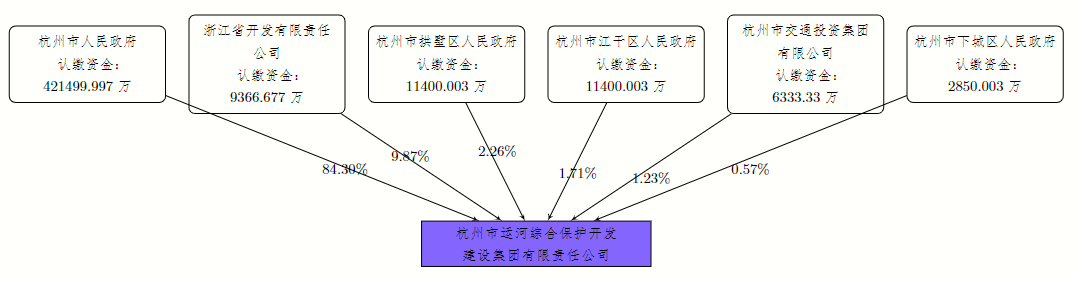
\includegraphics[width=0.75\textwidth]{img7.png}} \\
        \midrule 
        控股子公司 & \multicolumn{3}{p{11cm}|}{
        截至目前共有15家一级控股子公司(2021年12月17日天眼查查询),明细如下(单位: 万元):
    \end{longtable}
    }
\end{lstlisting}
但命令 \colorbox{lightgray}{longtable} 中可以设置 \colorbox{lightgray}{multicol},并且每一列也可以再插入
一个表格,也就是 \colorbox{lightgray}{tabular},新的表格不可以再跨页,所以,我们需要记住位置,当新的表格已经
达到页尾,我们再在新的一页中插入新的 \colorbox{lightgray}{multicol},并且在新的列中,接着上文所建立的表格,
再建立一个新的 \colorbox{lightgray}{tabular},写新的内容。

\section{存在不足}
总结存在的不足,主要是加强业务知识学习与克服自身缺点。
\par 
第一,缺少自制力。主要体现在两个方面,首先,要加强理智处理事情的能力,要培养团队意识,不给大家和小组造成麻烦,
培养大局意识。其次,做事不能抓住主要矛盾,对工作缺乏合理的安排,眉毛胡子一把抓。什么都要做好的结果,只能是什么
都做不好。分不清主次,反而耽误了时间、拖慢了团队的工作效率。
\par 
第二,加强沟通。与大家合作要坦诚、信任,有效沟通不仅能消除矛盾,还融洽了关系、提高工作效率,在写作评审报告中,
暴露出来的问题,主要就是没有即使沟通引起的,以后要加强与领导、同事沟通。
\par
第三,加强自身学习,积累工作经验,改进工作方法,向周围的同事学习,重点学习他们在面对问题时做的判断、处理事情的方法、
积极面对困难的勇气。查找不足,道阻且长,要有担当,不要害怕面对困难。
\section{结语}
最后,还是感谢领导与同事们对我的支持与帮助,我深知自己还存在许多缺点与不足,业务知识不够熟悉,工作方式不够成熟,
沟通经验不多丰富。这些都让我更加了解自己,我要努力克服这些缺点,尽职尽责做好每一件事。
\newpage 
\begin{appendices}
    \subfile{Appendix1.tex}
    \newpage 
    \subfile{Appendix2.tex}
\end{appendices}
\end{document}